Der \emph{Enable}-Eingang des LT3741 wird einerseits vom Mikrocontroller mit dem
$BUCK\_EN$  Signal ein- und ausgeschalten, anderseits  wird  der  Enable-Eingang
auch mit vorrang in Hardware ausgeschalten, falls  die  \SI{36}{\volt}  Spannung
unter $\approx  \SI{25}{\volt}$  sinken w\"urde. Dies erlaubt ein kontrolliertes
und vorhersehbares Verhalten  des LT3741 w\"ahrend Ein- und Ausschaltvorg\"angen
des Endproduktes. Die Schaltung dazu ist in der Abbildung \ref{fig:circuit:uvlo}
ersichtlich.

\begin{figure}[th!]
    \center
    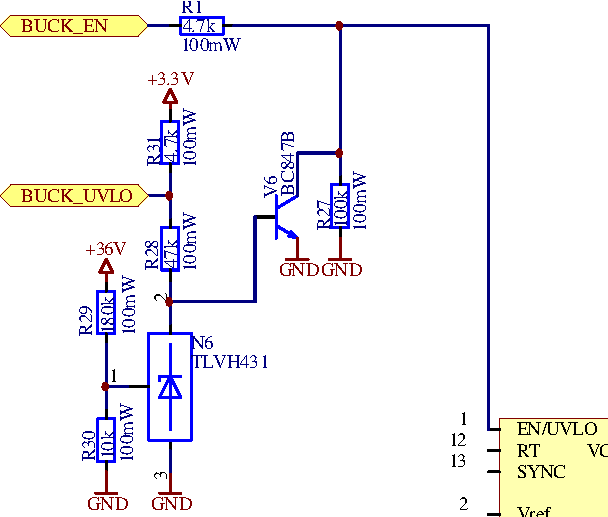
\includegraphics[width=.6\textwidth]{images/circuit/uvlo.pdf}
    \caption{Under-Voltage Lock-Out (UVLO) erm\"oglicht ein kontrolliertes Ein- und Ausschalten des Reglers}
    \label{fig:circuit:uvlo}
\end{figure}

Im Falle einer Unterspannung  wechselt  $N_6$  in den sperrenden Zustand \"uber,
der  Transistor $V_6$ beginnt zu leiten, und der  Enable-Eingang  wird  auf  Low
gezogen.  Die  Spannung  an  $BUCK\_UVLO$  triggert  beim  Mikrocontroller   ein
Interrupt.
